\section{Arquitectura de la API}\label{sec:arquitectura-laura}
\subsection{Separación de responsabilidades}
La organización por capas evita que una ruta mezcle autorización, reglas de negocio y consultas SQL. Express permite asociar rutas y middleware con los métodos HTTP~\cite{express}. La Fig.~\ref{fig:arquitectura-laura} resume la dirección principal de las dependencias.
\begin{figure}[!t]\centering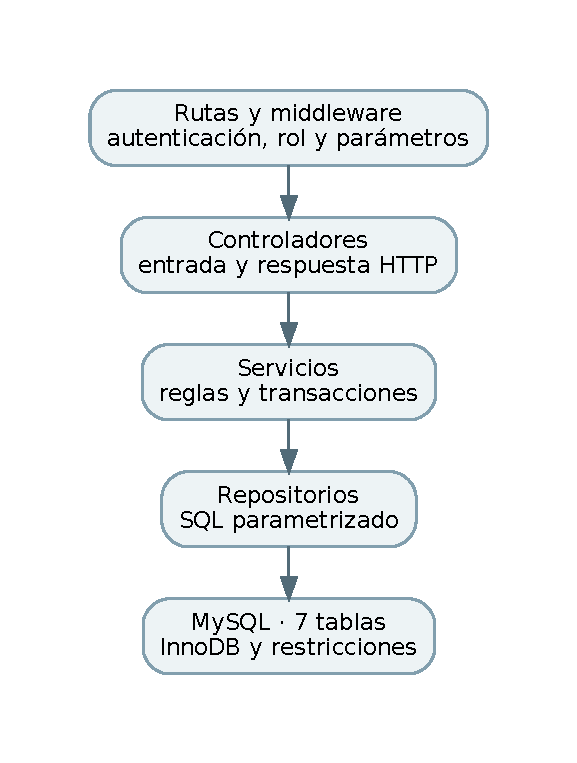
\includegraphics[width=.88\columnwidth,height=.42\textheight,keepaspectratio]{figuras/modelo/arquitectura.pdf}\caption{Capas de la API y persistencia.}\label{fig:arquitectura-laura}\end{figure}

\texttt{routes} declara recursos, métodos y controles de acceso. \texttt{controllers} convierte parámetros HTTP y selecciona respuestas. \texttt{services} aplica las reglas del gimnasio: cupos, horarios, propiedad, asistencia y protección del historial. \texttt{repositories} contiene SQL parametrizado y los alias de salida. \texttt{config} concentra conexión y variables de entorno; \texttt{utils} reúne validaciones y fechas comunes.

\subsection{Controles comunes}
El middleware valida el JWT y consulta la cuenta actual: un token existente no permite usar una cuenta desactivada. Los controles de rol y propiedad se combinan; conocer un identificador no concede acceso. El registro público asigna el rol \texttt{client} y rechaza un campo de rol enviado por el solicitante. Las credenciales y tokens se excluyen de las respuestas de perfil y se ocultan en las evidencias.

El manejador central de errores convierte conflictos y errores esperables en respuestas uniformes. Una excepción no controlada produce una respuesta genérica; los detalles SQL no se exponen al cliente. Esto mantiene el formato HTTP sin repetir el mismo manejo en cada controlador.

\subsection{Persistencia y concurrencia}
\texttt{database.js} administra el pool de conexiones y fija UTC en las operaciones. Los servicios que necesitan atomicidad reciben una conexión transaccional y la pasan al repositorio. Una reserva bloquea la fila de la clase antes de contar cupos: la lectura y la inserción pertenecen a la misma transacción. Las restricciones de unicidad y de referencia agregan protección a las validaciones de aplicación.

No se permite que el cliente escriba SQL ni determine el precio pagado. La configuración se obtiene del entorno; \texttt{.env.example} documenta sus nombres sin guardar credenciales reales. La documentación interactiva y el contrato se sirven desde la aplicación en \texttt{/docs} y \texttt{/openapi.json}.
